\section{The Particle Flow Algorithm}


\todo{Rework and resume the PF chapter}
The information available from all CMS subdetectors is employed in the particle-flow (PF) algorithm \cite{CMS:2009nxa,CMS:2010byl} to identify and reconstruct individual particles in the event, namely muons, electrons, photons, and charged and neutral hadrons. These particles are used to reconstruct jets, \hadtau candidates, and the vector imbalance in transverse momentum in the event, referred to as \ptvecmiss, as well as to quantify the isolation of leptons. 

Electrons are reconstructed by matching tracks in the inner detector with energy depositions in the ECAL [38, 42]. The tracks of electron candidates are reconstructed using a Gaussiansum filter [43] algorithm, which accounts for the emission of bremsstrahlung photons along the electron trajectory. Energy loss in bremsstrahlung is reconstructed by searching for energy depositions in the ECAL located in directions tangential to the electron track. A multivariate approach based on boosted decision trees (BDT) [44] is employed for electron identification [45]. The identification of muons is based on linking track segments reconstructed in the silicon tracking detector and in the muon system [46]. The matching between track segments is done outside-in, starting from a track in the muon system, and inside-out, starting from a track reconstructed in the inner detector. In case a link can be established, the track parameters are refitted using the combined hits in the inner and outer detectors, with the resulting track referred to as a global muon track. Quality criteria are applied on the multiplicity of hits, on the number of matched segments, and on the fit quality of the global muon track, quantified through a \ensuremath{\chisquare}.

Electrons and muons originating from decays of W and Z bosons are expected to be isolated, while leptons from heavy flavour (charm and bottom quark) decays, as well as from in-flight decays of pions and kaons, are often reconstructed within jets. The signal is distinguished from multijet background through the sum of scalar pT values of charged particles, neutral hadrons,and photons,reconstructed within a cone of size ∆R = √(∆η)2 + (∆φ)2 of 0.4,centered around the lepton direction, using the PF algorithm. Neutral hadrons and photons within the innermost region of the cone are excluded from the sum, to prevent the footprint of the lepton in ECAL and HCAL from causing the lepton to fail isolation criteria. Charged particles close to the direction of electrons are also excluded from the computation, to avoid counting tracks from converted photons emitted by bremsstrahlung. Efficiency loss due to pileup is kept minimal by considering only charged particles originating from the lepton production vertex in the isolation sum. 

Collision vertices are reconstructed using a deterministic annealing algorithm [47, 48]. The reconstructed vertex position is required to be compatible with the location of the LHC beam in the x-y plane. The primary collision vertex (PV) is taken to be the vertex that maximizes ∑tracks p2 T. The sum extends over all tracks associated with a given vertex.

Jets within the range |η| < 4.7 are reconstructed using the anti-kT algorithm[35] with a distance parameter of 0.5. As mentioned previously,the particles reconstructed by the PF algorithm are used as input to the jet reconstruction. Reconstructed jets are required not to overlap with identified electrons, muons, or τh within ∆R < 0.5, and to pass two levels of jet identification criteria: (i) misidentified jets, mainly arising from calorimeter noise, are rejected by requiring reconstructed jets to pass a set of loose jet identification criteria [49] and (ii) jets originating from pileup interactions are rejected through an MVA-based jet identification discriminant, relying on information about the vertex and energy distribution within the jet[50]. The energy of reconstructed jets is calibrated as a function of jet pT and η [51]. The contribution of pileup to the energy of jets originating from the hard scattering is compensated by determining a median transverse momentum density (ρ) for each event, and subtracting the product of ρ times the area of the jet, computed in the η−φ plane,from there constructed jet pT [52,53]. Jets originating from the hadronization of b quarks are identified through the combined secondary vertex (CSV) algorithm[54], which exploits observables related to the long lifetime of b hadrons and the higher particle multiplicity and mass of b jets compared to light-quark and gluon jets.

Two algorithms are used to reconstruct \ptvecmiss , the imbalance in transverse momentum in the event, whose magnitude is referred to as \met . The standard algorithm computes the negative vectorial sum of all particle momenta reconstructed using the PF algorithm. In addition, a multivariate regression algorithm[37] has been developed to reduce the effect of pileup on the resolution in \met. The algorithm utilizes the fact that pileup predominantly produces jets of low pT, while leptons and high-pT jets are produced almost exclusively in the hard-scatter. The transverse mass, \mt, of the system constituted by an electron or a muon and \met is used to either select or remove events that are due to W+jets and tt production. 

\begin{figure}
	\centering
	\begin{subfigure}{1\textwidth}
		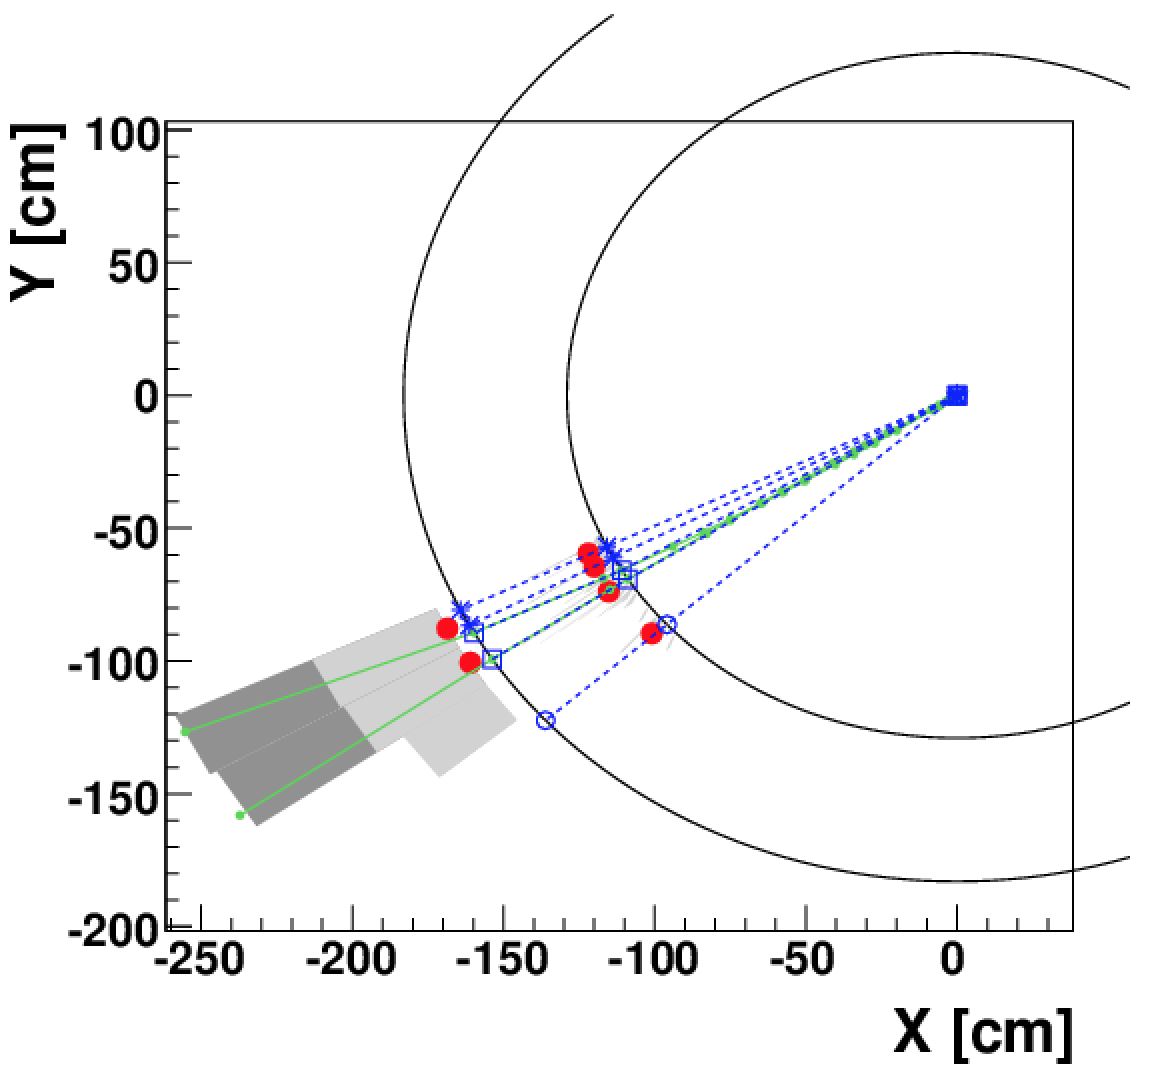
\includegraphics[width=.8\linewidth]{analysis/pics/PF_a.png}
		\caption{The $(x, y)$ view.}
		\label{fig:PF_a}
	\end{subfigure}
	
	\begin{subfigure}{.4\textwidth}
		\centering
		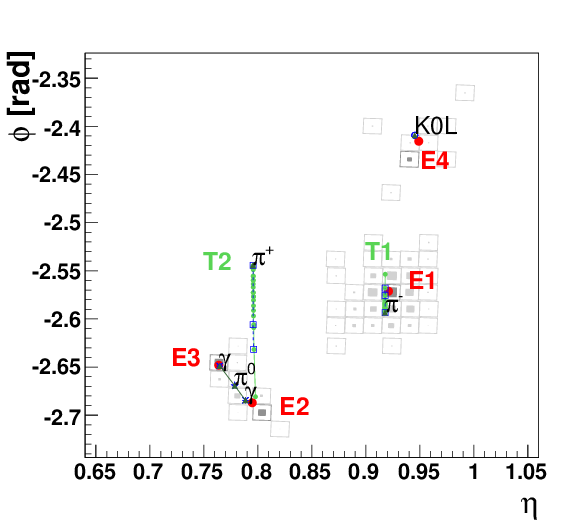
\includegraphics[width=.8\linewidth]{analysis/pics/PF_b.png}
		\caption{The $(\eta,\phi)$ view on ECAL.}
		\label{fig:PF_b}
	\end{subfigure}
		\begin{subfigure}{.4\textwidth}
			\centering
			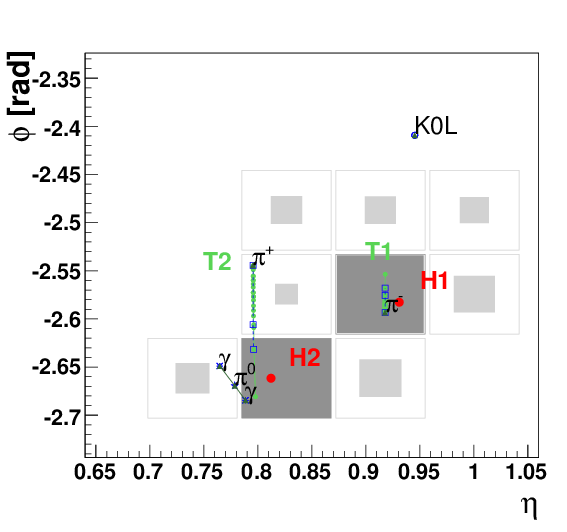
\includegraphics[width=.8\linewidth]{analysis/pics/PF_c.png}
			\caption{The $(\eta,\phi)$ view on HCAL.}
			\label{fig:PF_c}
		\end{subfigure}%
	\caption{An event display of a simple hadronic jet in the $(x, y)$ view (Figure \ref{fig:PF_a}) and in the $(\eta,\phi)$ view, where $\eta$ stands for pseudo-rapidity and $\phi$ for the azimuthal angle, on the ECAL surface (Figure \ref{fig:PF_b}) and the HCAL surface (Figure \ref{fig:PF_c}). (These two surfaces are represented as two circles centred around the interaction point in the first view.) The $K^{0}_{L}$, the $\pi^{-}$ and the two photons from the $\pi^{0}$ decay are detected as four well separated ECAL clusters (Figure \ref{fig:PF_b}). The $\pi^{+}$ leaves no energy in the ECAL. The two charged pions are reconstructed as charged-particle tracks, appearing as vertical solid lines in the $(\eta,\phi)$ views and circular arcs in the $(x, y)$ view. These tracks point towards two HCAL clusters (Figure \ref{fig:PF_c}). In all three views, the cluster positions are represented by dots, the simulated particles by dashed lines, and the position of their impact on the calorimeter surfaces by various open markers.}
	\label{fig:PF_event_display}
\end{figure}

\clearpage

\section {The Tau Lepton reconstruction}

The $\tau$ lepton was discovered between 1974 and 1977 by the team under Martin Perl while studying the $e^{+}+e^{-}\longrightarrow e^{\pm}+\mu^{\mp}$. With a mean lifetime of $2.9\times10^{−13}$ s and a mass of 1776.82 \mev \cite{Agashe:2014kda} is the heaviest of the leptons, enough to decay into hadrons, and it does so in about two thirds of the cases, typically into either one or three charged pions or kaons and up to two neutral pions \ensuremath{\pi^{0}}, and one neutrino \ensuremath{\nu_{\tau}}. The \ensuremath{\pi^{0}} meson decays almost exclusively into \ensuremath{\gamma\gamma}. Among all the possible hadronic decays as shown on Table \ref{table:tau_hdecay} the ones called "one-prong", where only one charged hadron is produced, are the most frequent. The $\tau$ decays also leptonically, with a branching ratio of $17\%$ for each channel, via the following decay $\tau\longrightarrow\nu_{\tau}W^{*}\longrightarrow\nu_{\tau}l\nu_{l}$.

\begin{figure}[tbh!]
	\begin{center}	
		\begin{tabular}{ | c | c | c | c |}
			\hline
			Decay Mode & Resonance & Mass [\mev] & BF (\%) \\ \hline
			\hline
			$\tau^{-}\longrightarrow h^{-}\nu_{\tau}$& $\pi$ & 139.6 & 11.6 \\ \hline
			$\tau^{-}\longrightarrow h^{-}\pi^{0}\nu_{\tau}$& $\rho$ & 770 & 26.0 \\ \hline
			%				$\tau^{-}\longrightarrow h^{-}\pi^{0}\pi^{0}\nu_{\tau}$ & $a_{1}$ & 1200 & \\ 10.8 \hline
			$\tau^{-}\longrightarrow h^{-} h^{+} h^{-} \nu_{\tau}$& $a_{1}$& 1200 & 9.8 \\ \hline
			$\tau^{-}\longrightarrow h^{-} h^{+} h^{-} \pi^{0}\nu_{\tau}$& & & 4.8 \\ \hline
			other hadronic channels& & & 1.7 \\ \hline
			\hline
			total & & & 64.8 \\ \hline
			\hline
		\end{tabular}
		\caption{ Hadronic tau decay modes into either one or three charged hadrons h and potential $\pi_{0}$, and the corresponding branching fractions BF. Also shown are the intermediate resonances and their masses, which are used in some of the tau reconstruction algorithms.}
		\label{table:tau_hdecay}
	\end{center}
\end{figure}

\subsection{Algorithm for \hadtau reconstruction and identification}



\clearpage

\section {The Jet reconstruction}

